
\documentclass[oneside,english]{llncs}

\usepackage[T1]{fontenc}
\usepackage[utf8]{luainputenc}
\usepackage{float}
\usepackage{amsthm}
\usepackage{amssymb}
\usepackage{graphicx}
\usepackage{caption,subcaption}
\usepackage{subfig}
\usepackage{babel}
\usepackage{gensymb}
\makeatletter
\renewcommand\subsubsection{\@startsection{subsubsection}{3}{\z@}%
                       {-18\p@ \@plus -4\p@ \@minus -4\p@}%
                       {4\p@ \@plus 2\p@ \@minus 2\p@}%
                       {\normalfont\normalsize\bfseries\boldmath
                        \rightskip=\z@ \@plus 8em\pretolerance=10000 }}
\renewcommand\paragraph{\@startsection{paragraph}{4}{\z@}%
                       {-12\p@ \@plus -4\p@ \@minus -4\p@}%
                       {2\p@ \@plus 1\p@ \@minus 1\p@}%
                       {\normalfont\normalsize\itshape
                        \rightskip=\z@ \@plus 8em\pretolerance=10000 }}

\setcounter{secnumdepth}{3}

\begin{document}

\title{Road detection from a simple 2D Camera}
\author{Dwight Kerkhove, Tom Vande Wiele, Sarah Merckx, Bavo Huyghe}
\institute{Science in Information Engineering Technology, Ghent University (UGent)}

\maketitle

\begin{abstract}
This paper describes our proposed method for detecting the road ahead from a single 2D camera using a new technique with minimal spanning trees for road boundary detection. The result is further refined with classifiers based on local binary patters and clustering on saturation and lightness to remove obstacles.
\end{abstract}

\section{Introduction}

Road detection has become a popular research topic in the advent of the self driving car era. It is however a challenging problem due to the large amount of different scenarios that can come into play: roads can have different textures (asphalt, paved roads, ..), there are a variety of weather effects (fog, snow, rain, sun glare) which also affect the road (aquaplaning, strong shadows, ...). It comes to no surprise that the biggest advancements have been made on highways where the road is mostly uniform with clear road markings and less varying conditions over a short period of time. Furthermore, any false negative can have catastrophic results so all detection algorithms must have a huge safety margin while still being able to perform well.

In the real world, a variety of sensors such as LIDAR, proximity sensors and stereo vision cameras are used to obtain enough information of the surroundings. More sensors in a harsh outdoors environment means an increase in cost, so in this paper we attempt to detect the road solely from the input of a normal 2D camera. Using a combination of techniques we were able to detect the road fairly accurately in common scenarios.

A lot of prior work tries to tackle this problem: Strygulec et al. \cite{key-11} attempts to find the boundaries of the road by using a particle filter approach. This works well for clearly distinguished textures around the boundaries but fails when there is a smooth transition or lots of dirt. Zhou et al. \cite{key-12} uses a variant of k-means clustering on different color spaces followed by a curve fitting to detect the road, which works well for non urban roads. Yanqing et al. \cite{key-13} starts off with combining Otsu thresholding and Canny edge detection followed by a Hough transform to extract line segments before applying a Monte Carlo method. This approach works well for straight roads without much curvature but is less effective with more complex cases such as T-sections and roundabouts. 
%what are the results + explanation why they are good/bad

In this paper we describe a novel technique for detecting road boundaries that is not limited to straight roads and can handle noise relatively well. This resulting mask is then combined with 2 other classifiers to exclude obstacles and hazards from the mask.

%Overview of the different sections of the paper
In section \ref{Methodology} \nameref{Methodology} we describe the general approach and follow up with more detailed description of the various components. Afterwards we discuss the results of our tests on the 4 training data sets in section \ref{Results} \nameref{Results} and conclude in section \ref{Conclusion} \nameref{Conclusion}.

\section{Methodology}\label{Methodology}

Our approach consists of using multiple classifiers on the input image and combining the masks together to minimize the errors that individual classifiers would have made. We have created 3 classifiers: the lane detection tries to find the lane or full road boundary regardless of obstacles on the road, the texture classifier compares texture patches and the clustering classifier analyzes the absence of color (saturation and lightness) of each pixel. The latter two classifiers have a lot of false positives in the environment outside the road but accurately detect a sudden change on the road, often indicating an obstacle. The lane detection (with mask $m_{l}$) is considered a strong classifier, the texture classifier (with mask $m_{t}$) and clustering classifier (with mask $m_{c}$) are considered weaker and require a consensus on the pixels. In essence the final mask ($m_{f}$) boils down to $m_{f}=m_{l}\&(m_{t}|m_{c})$.

To build in a safety margin we also erode the top of the mask a number of times. A high number of steps will increase the margin and reduce the possibility of classifying an obstacle or hazard as free road but at the cost of lowering the  overall performance.

\subsection{Lane detection}

The goal of the lane detection classifier is to create an initial contour of the lane or road, regardless of obstacles on the road. The classifier assumes that the car is already on the road and inside its lane. The classifier attempts to detect the boundaries of the lane to prevent the car from steering off the road. A common technique is to use a Canny edge detector and detect straight lines with a Hough transform while limiting the angle of the slope to reduce the amount of incorrect results\cite{key-9}\cite{key-15}. Once lines are known they can be further combined and refined using RANSAC \cite{key-10}. While this works well for straight roads this technique is hard to apply on curves and roundabouts. We present an alternative approach that creates a path following the boundaries of the lane, one that also includes the road segments that are not necessarily straight.

\subsubsection{Edge detection}

The input can have a wide variety of different parameters: roads with different textures (asphalt, paved road, ...), different lighting conditions, presence of road marks, etc. To reduce the number of edges that will interfere with the road detection we first apply a strong localized Gaussian blur, favoring the blurred image in the horizontal center at the bottom and gradually interpolating between the blurred image and the original\footnote{Averaging all the ground truths together to determine the probability of a pixel belonging to the road and using that probability as the intensity of the blur might yield a more accurate localized blurring.}.
The top of the image is less detailed due to perspective, so we decrease the blur in the vertical direction as well to better retain the original information in the distance. This reduces the edges generated on the road from pavements while retaining the road border that lie more on the sides of the image. 
After this preprocessing step we apply a simple Canny edge detector to find all the edges in the image with an empirically chosen upper threshold, and a lower threshold which is only half the value of the upper threshold\footnote{An Otsu threshold could be an option for automatic threshold selection \cite{key-1} but it requires the input to have a distinct foreground/background separation, which is not always the case in images obtained from a moving vehicle.}.

The choice of a good threshold is rather difficult. Having a high threshold will reduce the artifacts significantly, as the weaker edges are omitted, but will cause the actual border of the road to be missed as well. In order to reduce the impact of a badly chosen threshold we find all the contours\footnote{Using OpenCV's findContours method} of the edges on the Canny image and leave only the "qualitative" edges. The edges we're most interested in are the boundaries of the road, which are usually long tendrils. We assign a penalty ($P_{c}$) to each contour based on the contours' density of pixels inside its bounding box and the approximation of the bounding box being square (aspect ratio closer to 1):\\
\\
$P_{c} = \frac{\#pixels\:of\:contour}{area_{bbox}} \times ratio_{bbox}$ with $ratio_{bbox} < 1$.\\
\\We then normalize all values to a [0-1] range and select only the contours with a low penalty (figure \ref{fig:Canny-Penalty-Method}). This allows us to reduce the Canny upper threshold while preventing noise to be accepted as an edge (figure \ref{fig:Canny-Contour-Output}) but at a computational cost that can rise rapidly the more noise is present.

When using a high enough fixed Canny upper threshold the edges toward the top of the image will be missed. Lowering the Canny upper threshold to include those edges will introduce noise edges at the bottom of the image. While most of these are random noise and are filtered out using the method described above, this is not the case when the edges come from a strong textured image, such as paved roads. These edges have the same properties as the edge of the road and will interfere with the correct boundary detection. 

We use an adaptive Canny upper threshold that is stepwise reduced toward the top of the image. Pixels further along the road contain a bigger area of the environment and will have a more averaged result, which reduces the texture and magnitude of potential edges. This means that a lower Canny upper threshold will still be able to detect the reduced local maxima in the magnitudes, but will not introduce edges from texture anymore. This approach also has the advantage that noise will be much less likely to occur, and as such reduce the computational impact of the above filtering.

\begin{figure}
    \centering
    \begin{subfigure}[b]{.4\textwidth}
        \includegraphics[width=\textwidth,height=5cm]{canny_contourspenalty}
        \caption{Penalty method (green has low penalty score, red has high score.).} \label{fig:Canny-Penalty-Method}
    \end{subfigure}\qquad
    \begin{subfigure}[b]{.4\textwidth}
        \includegraphics[width=\textwidth,height=2cm]{canny_contourinputframe}
        \caption{Input frame}\label{fig:Canny-Contour-Input}
        \vspace{1ex}
        \includegraphics[width=\textwidth,height=2cm]{canny_treshold15_contourpenalty15}
        \label{fig:Canny-Contour-Output}
        \caption{Noisy contours (color) are not part of the accepted edges (white).}
    \end{subfigure}
\caption{Penalizing noisy contours allows for a lowering of the Canny upper threshold.}
\end{figure}
%
\subsubsection{Detecting boundaries of the lane}
To detect the boundaries we use a technique similar to photon mapping, used extensively in global illumination \cite{key-4}. The general idea is to shoot rays ("photons") from the light sources, let them bounce around in the scene and save the intersection points and their color. This creates a point cloud that can be used as an indirect lighting reference. In our approach we select a number of starting points at the bottom of the image - points that are assumed to be on the road - and shoot a number of rays from each of those points over an arc of 180\degree. We then collect the intersection points with the Canny image for each ray (figure \ref{fig:Rays-shot-from}), determine the normal vector of the edge in that point and let the ray reflect to obtain a next intersection point. This can be recursively repeated until the maximum recursion depth threshold is reached (figure \ref{fig:A-single-ray}).
Having rays hit the road indirectly improves the boundary detection in areas where the boundary can't be reached by the direct rays\footnote{For example T sections or roundabouts have areas that can't be reached directly when rays are shot from the bottom of the image.}. In practice the image can be easily traversed using a Bresenham's line algorithm \cite{key-2} until a nonzero pixel is encountered in the Canny image. To determine the normal vector we apply a Sobel operator to obtain the slope $s=\frac{G_{y}}{G_{x}}$ with $G_{x}$ and $G_{y}$ as the gradients in x and y directions respectively. 
The normal vector is simply $\overrightarrow{n}=\left\{ 1,s\right\} $. When both the normal vector $\overrightarrow{n}$ and the incoming ray direction vector $\overrightarrow{d}$ are normalized the reflected vector can be calculated using $\overrightarrow{v}=\overrightarrow{d}-2(\overrightarrow{d}\cdot\overrightarrow{n})\overrightarrow{n}$.
With this new vector as direction vector and the intersection point as the new starting point\footnote{To avoid self intersection in the same point the starting point should be offset along the direction vector.} we can construct a new ray and repeat the process recursively.

\begin{figure}
    \centering
    \begin{subfigure}[t]{0.46\textwidth}
        \centering
        \includegraphics[width=1\textwidth]{lanedetector_rays}
        \caption{Rays shot from 3 starting points at the bottom with their first intersection hit point.}
        \label{fig:Rays-shot-from}
    \end{subfigure}
    \hfill
    \begin{subfigure}[t]{0.46\textwidth}
        \centering
        \includegraphics[width=1\textwidth]{lanedetector_reflection}
        \caption{A single ray shot bounced around the scene to create intersection points in the contour of the road (green), reaching an area that would otherwise be much less represented. The normals are shown in red.}
        \label{fig:A-single-ray}
    \end{subfigure}%
\caption{Path tracing on the Canny image.}
\vspace{-2em} % spacing required to negate padding after caption
\end{figure}

\subsubsection{Obtaining a closed path to mark on the mask}
We now have many hit points, mostly lying on the boundaries of the lane. Due to holes in the Canny image or objects on the road, it's possible that there are outlier hit points that don't match the border of the lane/road. When sufficient rays are cast much more hit points will be on the border and close together. We build a graph with all the hit points as nodes. Graph edges are created between neighbouring nodes within a predefined distance ($distance(n_{i},n_{j}) \leqslant T_{D}$). We then build a minimum spanning tree (MST) with Prim's algorithm \cite{key-5} using a point close to the bottom row as root and keep track of the deepest node
\footnote{A minimum spanning tree based on distances between the nodes is often called an Euclidean Minimum Spanning Tree (EMST), which have algorithms that are more efficient than the more general Prim's algorithm.}. Once the algorithm is finished we can use that node to travel back to the root to obtain the deepest path in the MST. Because it's much more likely that points lie on the side of the lane, any offshoots to outliers will be branches in the spanning tree that won't be part of the deepest path (\ref{fig:Deepest-path-from}). In order to have a closed fill-able path we then add the projection of the first and last point onto the bottom row as the new first and and new last point of the final path. Finally the resulting polygon can now be used to create a mask for the lane. (\ref{fig:The-closed-path}).

\begin{figure}
    \centering
    \begin{subfigure}[t]{0.46\textwidth}
        \centering
        \includegraphics[width=1\textwidth]{lanedetector_deepestpath}
        \caption{Deepest path from the minimum spanning tree is highlighted in red. Outliers on the left are ignored as desired.}
        \label{fig:Deepest-path-from}
    \end{subfigure}
    \hfill
    \begin{subfigure}[t]{0.46\textwidth}
        \centering
        \includegraphics[width=1\textwidth]{lanedetector_result}
        \caption{The filled closed path.}
        \label{fig:The-closed-path}
    \end{subfigure}%
\caption{Finding the boundaries of the lane by looking for the deepest path in a MST.}
\end{figure}

\subsubsection{Further optimizations}

This works fine with borders of any shape that are continuous, which is not always the case for road marks. Any hole large enough will let rays pass outside the boundary of the road and create outliers. We solve this problem with a Hough preprocessing step. After the Canny image is generated we detect the straight lines using a Hough Transform while limiting the angle of the resulting line slopes. Small gaps between line segments that are in line with each other will be bridged. We then draw the segments on the Canny image so the gaps are closed.

\subsubsection{Limitations}
While this works well, it will only detect the outline of the lane/road. Any obstacles on the road that are small enough will be hit by rays but represent only a tiny branch in the MST compared to the path to the deepest leaf. Other classifiers should be used to detect actual obstacles on the road.\\
When the Canny edges have too many false positives (for example edges between sunny and shadowed areas) or false negatives (due to a badly chosen Canny threshold) the performance of this classifier will decrease dramatically. Shadows should be removed as much as possible before the Canny edge detection. Because the vehicle is in motion any shadow removal technique based on excluding shadowed areas from the foreground after a foreground-background separation is unlikely to work \cite{key-6}. Qi Wu et al. proposes a method to remove shadows with patch based shadow edge detection \cite{key-3} that would work much better in these conditions.

\subsection{Road texture detection}
Roads have a distinct texture that differs significantly from the obstacles on them. There are a variety of ways for detecting and comparing the textures of patches. A Gabor filter bank can be built from training sets, patches can be compared with co-occurrence matrices or distances between their respective histograms of binning local binary patterns (LBP) \cite{key-14}. We chose the latter because it's the least light sensitive and doesn't require building a training set in advance. The LBP codes are calculated for each pixel in the image using the neighbouring pixels. We also apply a slight offset to the center pixel value to reduce the fluctuations of bit values. Afterwards we divide the image into cells or patches of a fixed size\footnote{Depending on the use case we had the best results with a patch size of 8x8 or 16x16.}. All these patches are then compared to the patches in the middle of the bottom row of the image (which is assumed to be a road) by calculating the histogram of each one and comparing them with a Kullback-Leibler distance. If the patches are similar enough they will be accepted as part of the road. The patches from the reference row that are encountered most in the image will be kept aside to test against in future frames. This increases the accuracy slightly but increases the computational cost somewhat due to the extra comparisons.

\subsection{Detection using clustering of saturation and lightness}

Roads often differ from their environment in saturation and lightness. By finding clusters in a feature space consisting of those parameters we can separate the road from the environment and obstacles on the road. K-means is a popular approach for clustering but requires you to specify the number of clusters, something that is not always known beforehand. Mean shift\cite{key-7} is another clustering technique\footnote{Mean shift is also frequently used in computer vision for tracking objects over a number of frames.}
that uses a window with a certain radius around the centroid to group feature points and shift its cluster centroid to its stability point. Centroids that have overlapping windows can be merged together to reduce the number of clusters. While this is an effective approach for finding well defined clusters\footnote{Well defined in the sense that the points belonging to the same cluster are close enough together to fall within the selected window radius.} that exclude the outliers, it's also very slow because the algorithm starts off with each feature point being a cluster and gradually merging them together. We use an iterative approach alternating between k-means
\footnote{The first k-means centroid selection can be optimized using the k-means++ algorithm \cite{key-8}, which has a higher cost for selecting centroids but will converge much faster afterwards.} 
and mean shift which minimizes these individual issues. K-means is faster for scenarios with a lot of feature points and thus is used for the initial segmentation of the image into different clusters. Once the centroids are converged to their stable positions we use a mean shift clustering to optimize the cluster centroids and merge clusters with enough overlap together\footnote{We chose a threshold of 75\% empirically. If there is more overlap between the clusters they will be merged.}. We then repeat the process if the cluster count has been decreased. This repetition ensures that points that were previously assumed outliers due to the position of the cluster centroids are reevaluated with the k-means step and either remain rejected or become part of a cluster with the next mean shift step.

Once all the pixels in the the image are clustered (or rejected as outliers) we can select the clusters that are most likely to contain the road pixels. As before, we assume that the vehicle is on the road and pixels at the bottom center are considered road pixels. In that bottom area we determine the cluster frequency and select the top clusters that have the highest frequency and are represented well enough. All pixels of the image that belong to these clusters can be considered road and are classified as such.

Clustering is problematic for real time systems since it requires multiple iterations of complexity $\mathcal{O}(n * k)$ (with k clusters and n pixels). While relatively few iterations are needed to converge to a stable state, it still takes a magnitude longer than other approaches. We increased the performance to more acceptable levels by downscaling the input frames and then applying morphological operations (dilate and erode) to fill small gaps in the generated mask.

\begin{figure}
    \centering
    \begin{subfigure}[t]{0.3\textwidth}
        \centering
        \includegraphics[width=1\textwidth]{clustering_input}
        \caption{The input frame}
        \label{fig:Clustering-input}
    \end{subfigure}
    \hfill
    \begin{subfigure}[t]{0.3\textwidth}
        \centering
        \includegraphics[width=1\textwidth]{clustering_scale4_radius_01}
        \caption{4x downscale factor and window radius of 10\% of the normalized feature space}
        \label{fig:Clustering-window10}
    \end{subfigure}%
    \hfill
    \begin{subfigure}[t]{0.3\textwidth}
        \centering
        \includegraphics[width=1\textwidth]{clustering_scale4_radius_005}
        \caption{Window radius of 5\%. More pixels are now interpreted as outliers.}
        \label{fig:Clustering-window5}
    \end{subfigure}%    
\caption{Clustering applied on an input frame with multiple road textures.}
\end{figure}


\section{Results}\label{Results}

We've tested our approach on 4 different sets of frames in 720p, each taken 1 second apart:
\begin{itemize}
    \item{Set 01} features a single lane with road markings in the middle to divide the road. It also contains a roundabout with the occasional cross roads and other marks for bus stops. 
    \item{Set 02} continues the route by turning onto a two lane road with well established road markings and a bit of traffic waiting for a stop light. The wet road has a higher than normal reflection.
    \item{Set 03} starts off with a separate single lane but narrows onto a smaller and gradually deteriorating asphalt road which have been fixed multiple times so it's a patchwork of different textures and colors. The car approaches the center of a town near the end with cars parked on both sides.
    \item{Set 04} takes place in a residential area with many tight corners and lots of paved roads with deep grooves. The road also has hard to distinguish boundaries in the distance towards the end.
\end{itemize}
    
To measure the performance of our approach we've created ground truths for each of the sets every 5 frames, for a total of 126 frames.

\begin{figure}
    \centering
    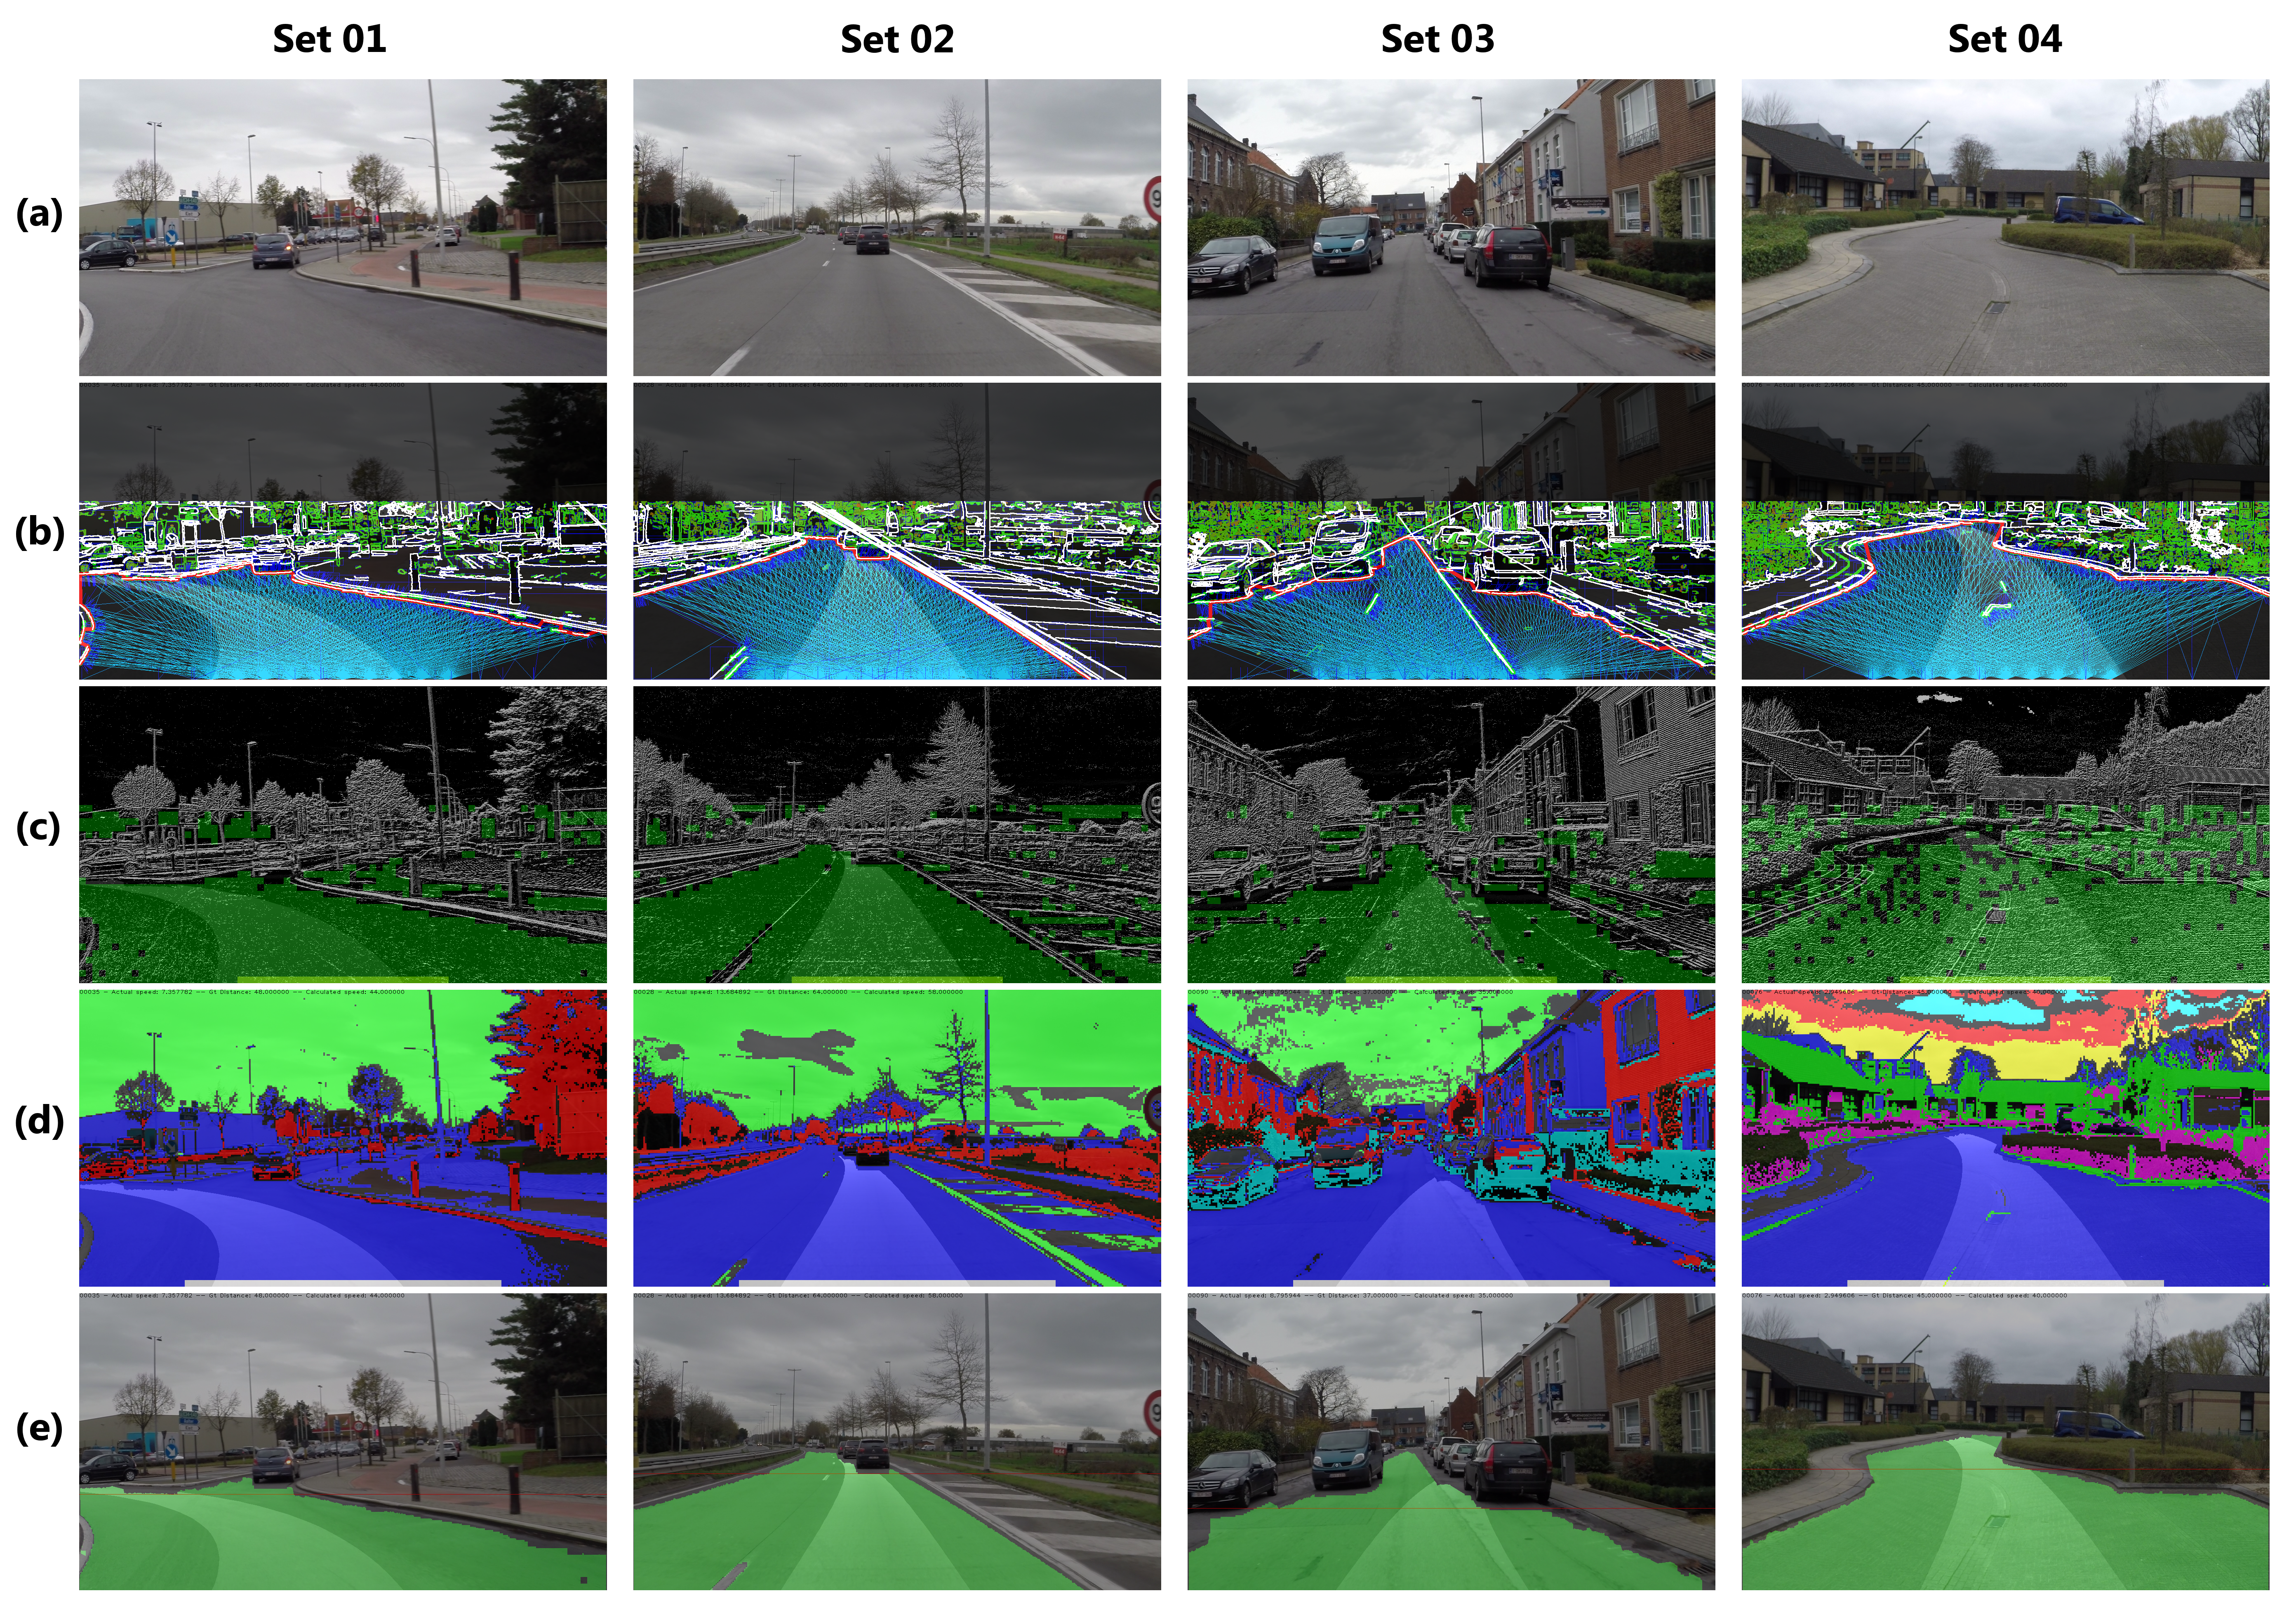
\includegraphics[width=0.97\textwidth]{setresults}
    \caption{Results: (a) Input frame (b) Lane detection, (c) Texture detection, (d) Clustering detection, (e) Final mask}
    \label{fig:Results}
\end{figure}

Finding a good starting Canny threshold proved to be tricky: the lane detection does a good job of ignoring most of the noisy edges by favoring the deepest path in the MST but has a tough time in set 04 with a low Canny threshold. The edges in the paved road are regular, long tendrils which won't be filtered out by the noise suppression. While the localized blurring helps in the center it still causes enough noise to have bad boundary detection. Increasing the Canny threshold is the only option to have a better detection rate, but that causes problems in set 03 and towards the end in set 04. The adaptive Canny threshold helps but isn't decreased fast enough to detect all the necessary edges from the lane boundary.

The texture detection also has problems with set 04, the bricks of the road near the bottom have a larger texture size than those further away, which causes mismatches when patches of both areas are compared.

The clustering detector makes sure set 04 still performs well but has problems with the road reflection in set 02. The pixels of the road in the distance deviate enough to become outliers of the main clusters.\\
By combining multiple classifiers the failure of one classifier can be compensated and allows us to classify the road correctly.

All three classifiers still have problems with roads markings such as cross roads or give-way road markings, which block the road ahead from being classified correctly. Soft and hard shadows are also a problem, especially when using adaptive Canny thresholds because the long contours of the shadows are easily detected as long continuous edges.

\begin{table}
    \begin{subtable}{.5\linewidth}
      \centering
        \begin{tabular}{ |c |c c c | c | } 
        \hline
         Set & TPR & FPR & F1-score & Average \\ 
          & \% & \% & & ms.\\ 
         \hline
     01 & 60.01 & 1.05 & 0.7362 & 319 \\ 
     02 & 88.83 & 5.93 & 0.9260 & 305 \\ 
     03 & 74.17 & 9.30 & 0.8380 & 282 \\ 
     04 & 69.92 & 5.18 & 0.8182 & 266 \\ 
     \hline
    \end{tabular}
    \caption{Threshold of 100.}
    
    \end{subtable}%
    \begin{subtable}{.5\linewidth}
      \centering
           \begin{tabular}{ |c |c c c | c | } 
         \hline
         Set & TPR & FPR & F1-score & Average \\ 
          & \% & \% & & ms.\\ 
         \hline
         01 & 59.49 & 0.07 & 0.7451 & 335 \\ 
         02 & 88.04 & 0.07 & 0.9346 & 317 \\ 
         03 & 70.07 & 7.41 & 0.8132 & 303 \\ 
         04 & 56.39 & 0.23 & 0.7193 & 314 \\ 
         \hline
        \end{tabular}
        \caption{Threshold of 50.}
    \end{subtable} 
    \caption{Performance comparison between 2 maximum Canny upper threshold values.}
    \label{tableresults}
    \vspace{-4em} % spacing required to negate padding after caption
\end{table}

As seen in table \ref{tableresults}, having a higher maximum for the Canny upper threshold causes more edges to be missed, resulting in a higher false positive rate (FPR). As expected, lowering the threshold has a big impact on the true positive rate (TPR) of set 04 due to its well textured roads. Other sets only have a slight decrease in the true positive rate while the false positive rate decreases significantly. The computational cost also rises slightly due to the increase in the amount of contours the algorithm has to check for filtering out noise, but generally stays around 3fps on a Intel Core i7-2630QM cpu from 2011. Because the road marks separating the lane in set 03 have a big gap between them the Hough lane assist is unable to add edges that prevent the mask from going outside the lane. This causes the high FPR on set 03, regardless of the chosen threshold.

To test the stability on a frame-to-frame basis we recorded a few 24fps videos\footnote{Results can be seen on \url{https://www.youtube.com/watch?v=e2uQc8CMpSE} and \url{https://www.youtube.com/watch?v=mK5Zu9gypnY}.} 
with a Lumia 630 phone from inside the car at rear mirror level. The image quality is much poorer than the previous sets: there is motion blur due to shaking, reflection from the windshield and overall much less contrast. Still our approach was able to correctly identify the boundaries of the road - regardless of road markings on the side - and exclude vehicles in front of the car from the final mask. Even in rainy conditions such as the wet road and reduced visibility our approach worked remarkably well. The final result was relatively stable, indicating that misdetection could be reduced by averaging the result of consecutive frames.

\begin{figure}[H]
    \centering
    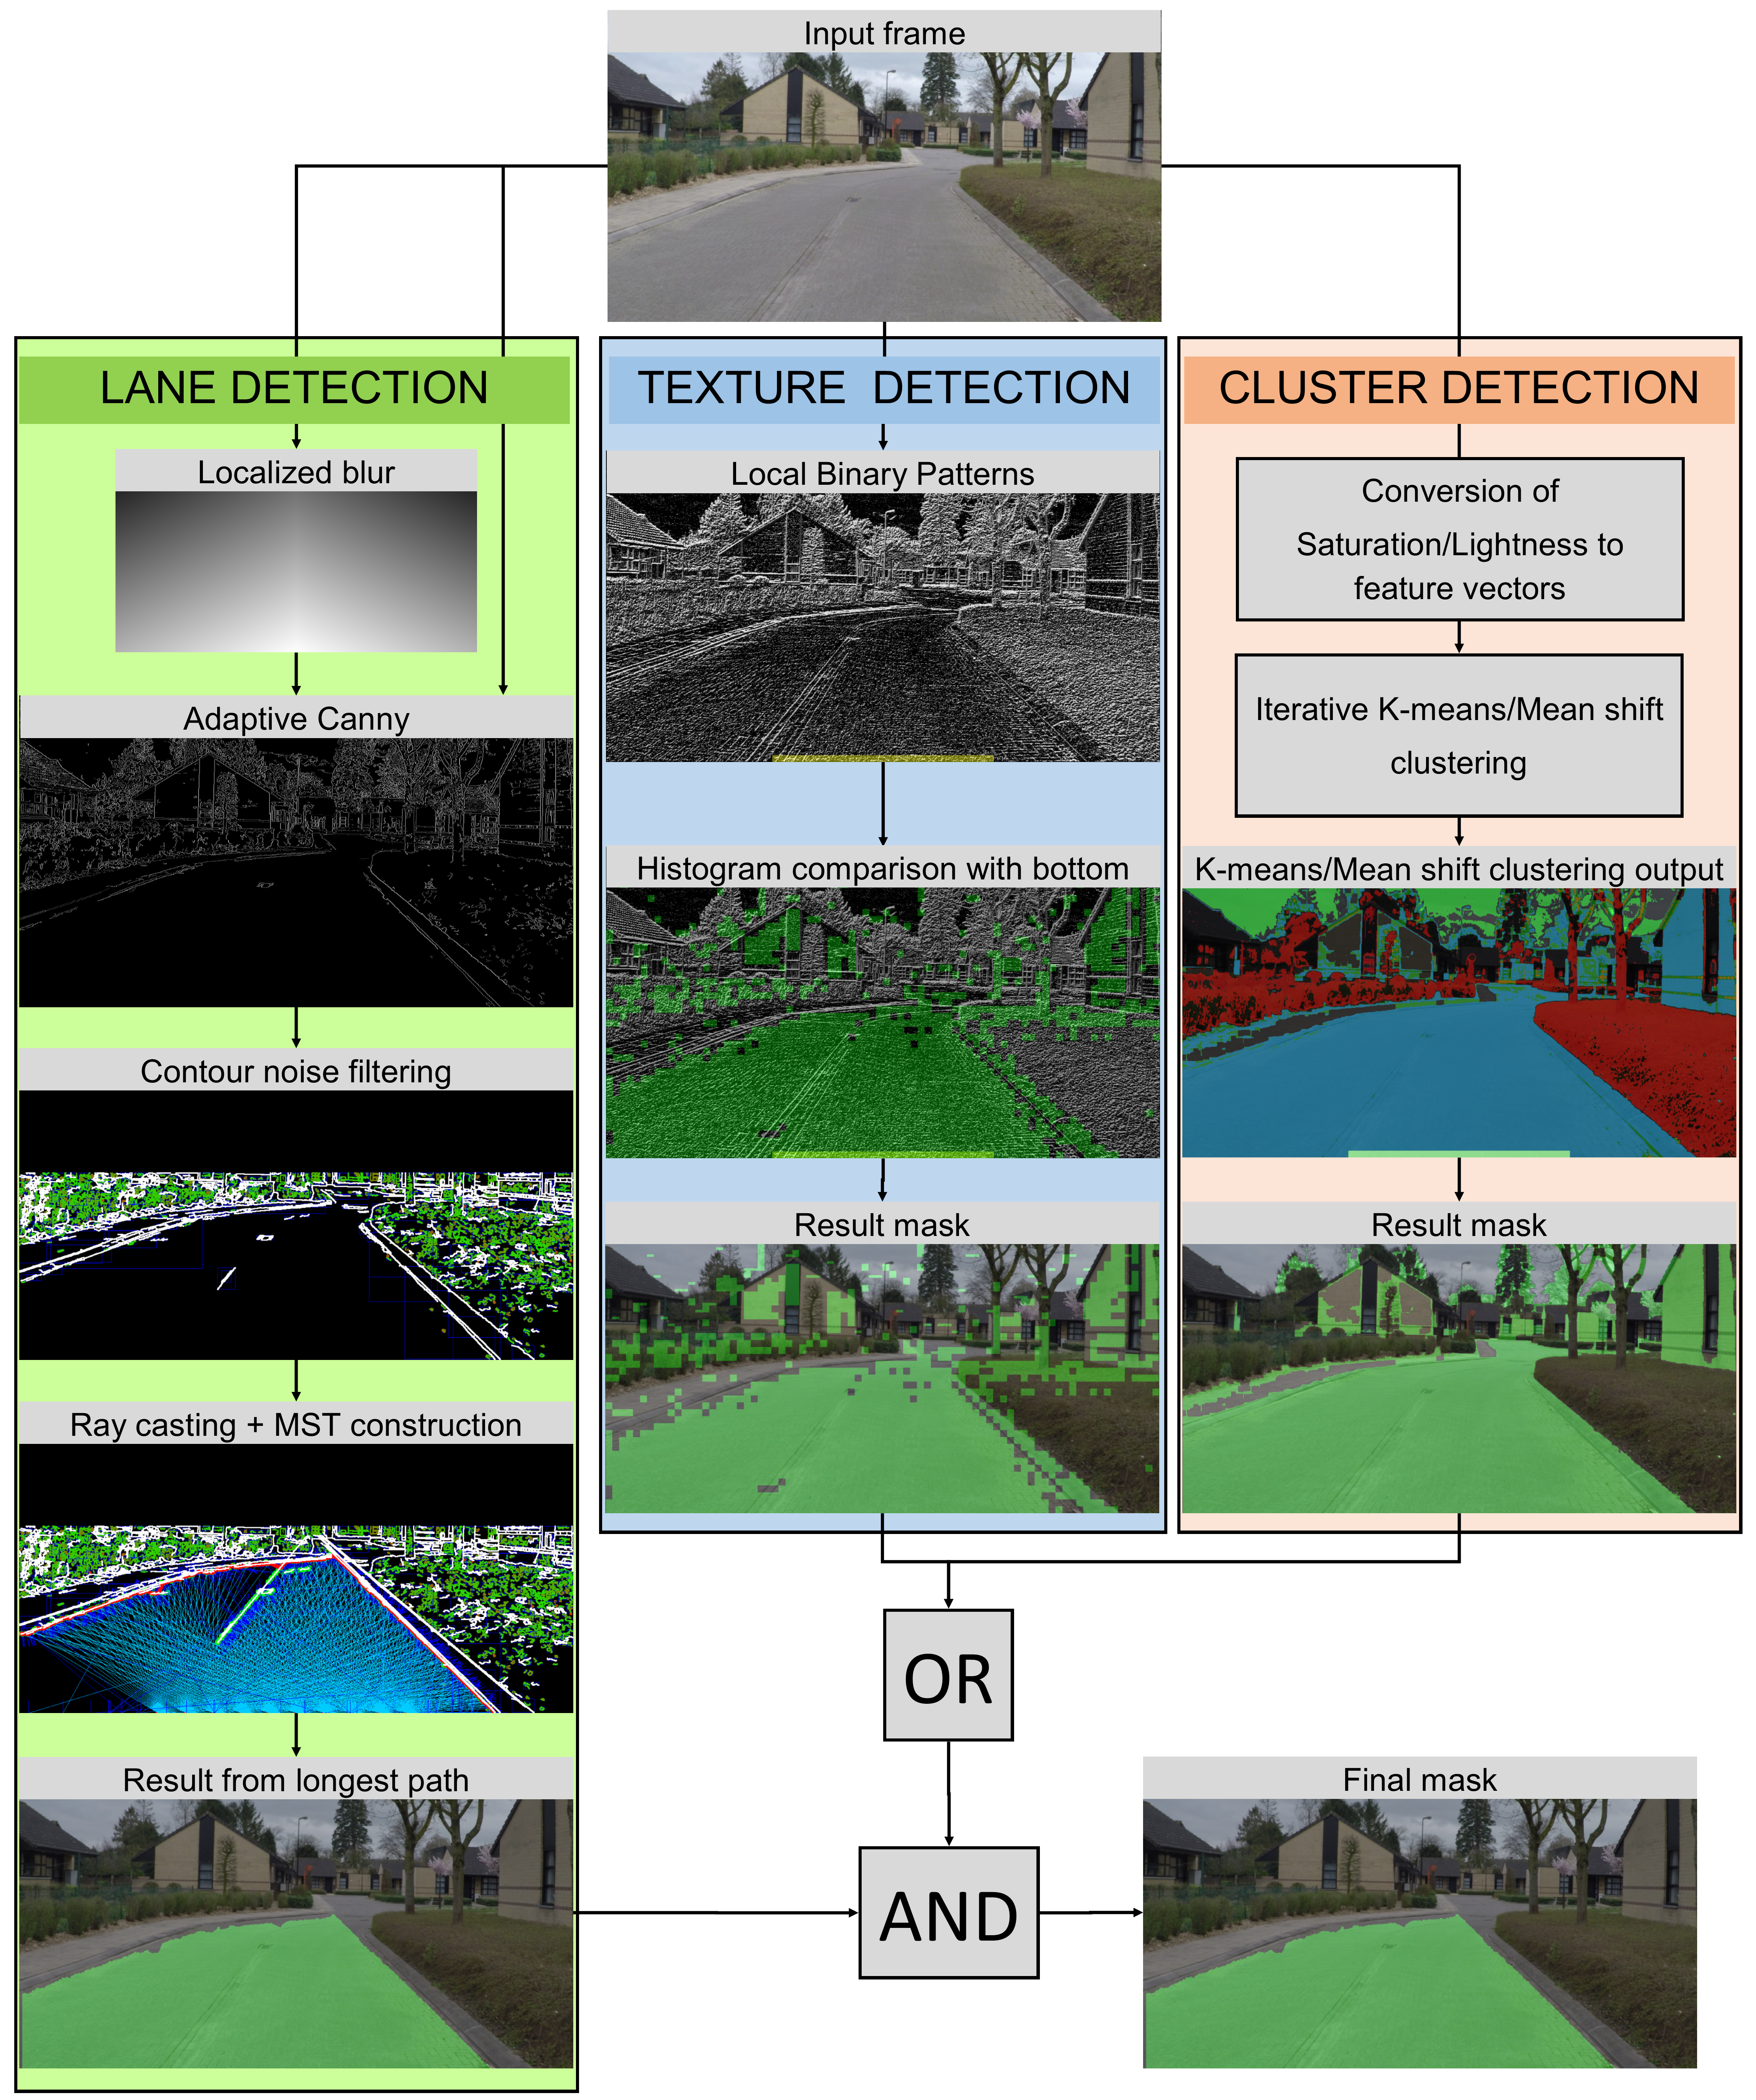
\includegraphics[height=13cm]{algorithmflow}
    \caption{Complete overview of our approach.
    \label{fig:AlgorithmOverview}}
    \vspace{-1em} % spacing required to negate padding after caption
\end{figure}

\section{Conclusion}\label{Conclusion}

In this paper we presented some novel techniques that can assist other approaches to detect road boundaries and obstacles on the road. The lane detection is effective with well defined Canny edges and has a certain degree of noise tolerance. By searching the deepest path it's not constrained to straight roads but its heavy reliance on edge detection can be a weak point. This problem is somewhat mitigated by making the Canny threshold adaptive.\\
Afterwards we described two more classifiers, one identifying texture similarity with LBP's and another that detects differences in saturation and lightness using iterative clustering. When both of these classifiers are in agreement the corresponding area is flagged as non-road. Based on our experiments we can conclude that our approach works well in most cases and is able to correctly identify the road ahead even in poor weather conditions but requires preprocessing to remove shadows and other unwanted edges.

\begin{thebibliography}{1}
\bibitem{key-1}Mei Fang, GuangXue Yue and QingCang Yu, The Study
on An Application of Otsu Method in Canny Operator, 2009.

\bibitem{key-2}Bresenham, J. E., Algorithm for computer control of
a digital plotter, 1965.

\bibitem{key-3}Qi Wu, Wende Zhang and B.V.K. Vijaya Kumar, Strong
Shadow Removal Via Patch-Based Shadow Edge Detection, 2012.

\bibitem{key-4}Jensen, H.W., 1996. Global illumination using photon maps. In Rendering Techniques’ 96 (pp. 21-30). Springer Vienna.

\bibitem{key-5}R. C. Prim, \textquotedbl{}Shortest connection networks
and some generalizations,\textquotedbl{} in The Bell System Technical
Journal, vol. 36, no. 6, pp. 1389-1401, Nov. 1957.

\bibitem{key-6}Sanin, A., Sanderson, C. and Lovell, B.C., 2012. Shadow
detection: A survey and comparative evaluation of recent methods.
Pattern recognition, 45(4), pp.1684-1695.

\bibitem{key-7}Fukunaga, K. and Hostetler, L.D., 1975. The estimation
of the gradient of a density function, with applications in pattern
recognition. Information Theory, IEEE Transactions on, 21(1), pp.32-40.

\bibitem{key-8}Arthur, D. and Vassilvitskii, S. (2007). \textquotedbl{}k-means++:
the advantages of careful seeding\textquotedbl{}. Proceedings of the
eighteenth annual ACM-SIAM symposium on Discrete algorithms. Society
for Industrial and Applied Mathematics Philadelphia, PA, USA. pp.
1027–1035.

\bibitem{key-9}Kang, D.J., Choi, J.W. and Kweon, I.S., 1996, September. Finding and tracking road lanes using “line-snakes”. In Intelligent Vehicles Symposium, 1996., Proceedings of the 1996 IEEE (pp. 189-194). IEEE.

\bibitem{key-10}Kuk, J.G., An, J.H., Ki, H. and Cho, N.I., 2010, September. Fast lane detection \& tracking based on Hough transform with reduced memory requirement. In Intelligent Transportation Systems (ITSC), 2010 13th International IEEE Conference on (pp. 1344-1349). IEEE.

\bibitem{key-11}Strygulec, S., Muller, D., Meuter, M., Nunn, C., Ghosh, S. and Wohler, C., 2013, July. Road boundary detection and tracking using monochrome camera images. In Information Fusion (FUSION), 2013 16th International Conference on (pp. 864-870). IEEE.

\bibitem{key-12}Zhou, L., Zhang, Y., Peng, D. and Wu, D., 2015. Improved K-means Clustering Color Segmentation for Road Perception.

\bibitem{key-13}Yanqing, W., Deyun, C., Chaoxia, S. and Peidong, W., 2010. Vision-based road detection by monte carlo method. Information Technology Journal, 9(3), pp.481-487.

\bibitem{key-14}Ojala, T., Pietikainen, M. and Harwood, D., 1994, October. Performance evaluation of texture measures with classification based on Kullback discrimination of distributions. In Pattern Recognition, 1994. Vol. 1-Conference A: Computer Vision \& Image Processing., Proceedings of the 12th IAPR International Conference on (Vol. 1, pp. 582-585). IEEE.

\bibitem{key-15}Fang, H., Yang, G.Q., Li, J., Shao, G.T., Zhang, C.Y. and Fu, C.G., 2016, February. An approach for road region detection. In Advanced Materials, Structures and Mechanical Engineering: Proceedings of the international Conference on Advanced Materials, Structures and Mechanical Engineering, Incheon, South Korea, May 29-31, 2015 (p. 93). CRC Press.

\end{thebibliography}

\end{document}